% ---------------------------------------------------------------------------
%  Suggestion: place in Section 4, where the descent is described
%  ("Proof of Theorem 1"), with \ref{fig:descent} in the text.
%  Generated from the certificate by gen_tikz.py; edit that, not this.
% ---------------------------------------------------------------------------
\begin{figure}[H]
\centering
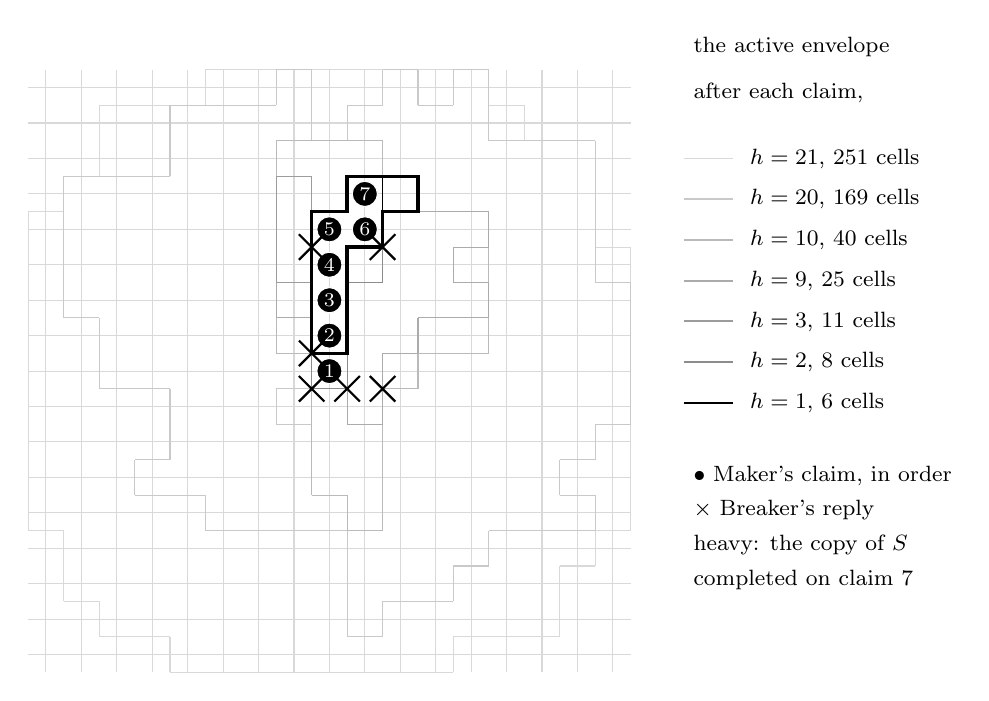
\begin{tikzpicture}[x=4.5mm,y=4.5mm,font=\small]
\draw[gray!30,step=1] (-.5,-.5) grid (16.5,16.5);
\draw[gray!30] (-0.5,3.5)--(0.5,3.5) (-0.5,3.5)--(-0.5,4.5) (-0.5,4.5)--(-0.5,5.5) (-0.5,5.5)--(-0.5,6.5) (-0.5,6.5)--(-0.5,7.5) (-0.5,7.5)--(-0.5,8.5) (-0.5,8.5)--(-0.5,9.5) (-0.5,9.5)--(-0.5,10.5) (-0.5,10.5)--(-0.5,11.5) (-0.5,12.5)--(0.5,12.5) (-0.5,11.5)--(-0.5,12.5) (0.5,1.5)--(1.5,1.5) (0.5,1.5)--(0.5,2.5) (0.5,2.5)--(0.5,3.5) (0.5,13.5)--(1.5,13.5) (0.5,12.5)--(0.5,13.5) (1.5,0.5)--(2.5,0.5) (1.5,0.5)--(1.5,1.5) (1.5,13.5)--(1.5,14.5) (1.5,15.5)--(2.5,15.5) (1.5,14.5)--(1.5,15.5) (2.5,0.5)--(3.5,0.5) (2.5,15.5)--(3.5,15.5) (3.5,-0.5)--(4.5,-0.5) (3.5,-0.5)--(3.5,0.5) (3.5,15.5)--(4.5,15.5) (4.5,-0.5)--(5.5,-0.5) (4.5,16.5)--(5.5,16.5) (4.5,15.5)--(4.5,16.5) (5.5,-0.5)--(6.5,-0.5) (5.5,16.5)--(6.5,16.5) (6.5,-0.5)--(7.5,-0.5) (6.5,16.5)--(7.5,16.5) (7.5,-0.5)--(8.5,-0.5) (7.5,16.5)--(8.5,16.5) (8.5,-0.5)--(9.5,-0.5) (8.5,16.5)--(9.5,16.5) (9.5,-0.5)--(10.5,-0.5) (9.5,16.5)--(10.5,16.5) (10.5,-0.5)--(11.5,-0.5) (11.5,-0.5)--(11.5,0.5) (10.5,16.5)--(11.5,16.5) (11.5,0.5)--(12.5,0.5) (11.5,16.5)--(12.5,16.5) (12.5,15.5)--(12.5,16.5) (12.5,0.5)--(13.5,0.5) (12.5,15.5)--(13.5,15.5) (13.5,14.5)--(13.5,15.5) (13.5,0.5)--(14.5,0.5) (14.5,0.5)--(14.5,1.5) (14.5,1.5)--(14.5,2.5) (13.5,14.5)--(14.5,14.5) (14.5,2.5)--(15.5,2.5) (15.5,2.5)--(15.5,3.5) (15.5,11.5)--(15.5,12.5) (15.5,12.5)--(15.5,13.5) (14.5,14.5)--(15.5,14.5) (15.5,13.5)--(15.5,14.5) (15.5,3.5)--(16.5,3.5) (16.5,3.5)--(16.5,4.5) (16.5,4.5)--(16.5,5.5) (16.5,5.5)--(16.5,6.5) (16.5,6.5)--(16.5,7.5) (16.5,7.5)--(16.5,8.5) (16.5,8.5)--(16.5,9.5) (16.5,9.5)--(16.5,10.5) (15.5,11.5)--(16.5,11.5) (16.5,10.5)--(16.5,11.5);
\draw[gray!42] (0.5,9.5)--(1.5,9.5) (0.5,9.5)--(0.5,10.5) (0.5,10.5)--(0.5,11.5) (0.5,11.5)--(0.5,12.5) (0.5,13.5)--(1.5,13.5) (0.5,12.5)--(0.5,13.5) (1.5,7.5)--(2.5,7.5) (1.5,7.5)--(1.5,8.5) (1.5,8.5)--(1.5,9.5) (1.5,13.5)--(2.5,13.5) (2.5,5.5)--(3.5,5.5) (2.5,4.5)--(3.5,4.5) (2.5,4.5)--(2.5,5.5) (2.5,7.5)--(3.5,7.5) (2.5,13.5)--(3.5,13.5) (3.5,4.5)--(4.5,4.5) (3.5,5.5)--(3.5,6.5) (3.5,6.5)--(3.5,7.5) (3.5,13.5)--(3.5,14.5) (3.5,15.5)--(4.5,15.5) (3.5,14.5)--(3.5,15.5) (4.5,3.5)--(5.5,3.5) (4.5,3.5)--(4.5,4.5) (4.5,15.5)--(5.5,15.5) (5.5,3.5)--(6.5,3.5) (6.5,6.5)--(6.5,7.5) (5.5,15.5)--(6.5,15.5) (6.5,3.5)--(7.5,3.5) (6.5,6.5)--(7.5,6.5) (6.5,7.5)--(7.5,7.5) (7.5,14.5)--(7.5,15.5) (6.5,16.5)--(7.5,16.5) (6.5,15.5)--(6.5,16.5) (7.5,15.5)--(7.5,16.5) (7.5,3.5)--(8.5,3.5) (7.5,6.5)--(7.5,7.5) (7.5,14.5)--(8.5,14.5) (8.5,0.5)--(9.5,0.5) (8.5,0.5)--(8.5,1.5) (9.5,0.5)--(9.5,1.5) (8.5,1.5)--(8.5,2.5) (8.5,2.5)--(8.5,3.5) (8.5,15.5)--(9.5,15.5) (8.5,14.5)--(8.5,15.5) (9.5,1.5)--(10.5,1.5) (9.5,16.5)--(10.5,16.5) (9.5,15.5)--(9.5,16.5) (10.5,15.5)--(10.5,16.5) (10.5,1.5)--(11.5,1.5) (11.5,1.5)--(11.5,2.5) (10.5,15.5)--(11.5,15.5) (11.5,2.5)--(12.5,2.5) (12.5,2.5)--(12.5,3.5) (12.5,14.5)--(12.5,15.5) (11.5,16.5)--(12.5,16.5) (11.5,15.5)--(11.5,16.5) (12.5,15.5)--(12.5,16.5) (12.5,3.5)--(13.5,3.5) (12.5,14.5)--(13.5,14.5) (13.5,3.5)--(14.5,3.5) (14.5,4.5)--(14.5,5.5) (13.5,14.5)--(14.5,14.5) (14.5,4.5)--(15.5,4.5) (14.5,3.5)--(15.5,3.5) (15.5,3.5)--(15.5,4.5) (14.5,5.5)--(15.5,5.5) (15.5,5.5)--(15.5,6.5) (15.5,10.5)--(15.5,11.5) (15.5,11.5)--(15.5,12.5) (15.5,12.5)--(15.5,13.5) (14.5,14.5)--(15.5,14.5) (15.5,13.5)--(15.5,14.5) (15.5,6.5)--(16.5,6.5) (16.5,6.5)--(16.5,7.5) (16.5,7.5)--(16.5,8.5) (16.5,8.5)--(16.5,9.5) (15.5,10.5)--(16.5,10.5) (16.5,9.5)--(16.5,10.5);
\draw[gray!54] (6.5,8.5)--(7.5,8.5) (6.5,8.5)--(6.5,9.5) (6.5,9.5)--(6.5,10.5) (6.5,10.5)--(6.5,11.5) (6.5,11.5)--(6.5,12.5) (6.5,12.5)--(6.5,13.5) (6.5,14.5)--(7.5,14.5) (6.5,13.5)--(6.5,14.5) (7.5,4.5)--(8.5,4.5) (7.5,4.5)--(7.5,5.5) (7.5,5.5)--(7.5,6.5) (7.5,6.5)--(7.5,7.5) (7.5,7.5)--(7.5,8.5) (7.5,14.5)--(8.5,14.5) (8.5,3.5)--(9.5,3.5) (8.5,3.5)--(8.5,4.5) (9.5,3.5)--(9.5,4.5) (9.5,4.5)--(9.5,5.5) (9.5,5.5)--(9.5,6.5) (9.5,6.5)--(9.5,7.5) (9.5,12.5)--(9.5,13.5) (8.5,14.5)--(9.5,14.5) (9.5,13.5)--(9.5,14.5) (9.5,7.5)--(10.5,7.5) (10.5,7.5)--(10.5,8.5) (9.5,12.5)--(10.5,12.5) (10.5,8.5)--(11.5,8.5) (10.5,12.5)--(11.5,12.5) (11.5,8.5)--(12.5,8.5) (12.5,8.5)--(12.5,9.5) (12.5,9.5)--(12.5,10.5) (12.5,10.5)--(12.5,11.5) (11.5,12.5)--(12.5,12.5) (12.5,11.5)--(12.5,12.5);
\draw[gray!66] (6.5,9.5)--(7.5,9.5) (6.5,9.5)--(6.5,10.5) (6.5,10.5)--(6.5,11.5) (6.5,11.5)--(6.5,12.5) (6.5,13.5)--(7.5,13.5) (6.5,12.5)--(6.5,13.5) (7.5,12.5)--(7.5,13.5) (7.5,7.5)--(8.5,7.5) (7.5,7.5)--(7.5,8.5) (7.5,8.5)--(7.5,9.5) (7.5,12.5)--(8.5,12.5) (8.5,6.5)--(9.5,6.5) (8.5,6.5)--(8.5,7.5) (9.5,6.5)--(9.5,7.5) (9.5,7.5)--(9.5,8.5) (8.5,13.5)--(9.5,13.5) (8.5,12.5)--(8.5,13.5) (9.5,12.5)--(9.5,13.5) (9.5,8.5)--(10.5,8.5) (10.5,8.5)--(10.5,9.5) (9.5,12.5)--(10.5,12.5) (10.5,9.5)--(11.5,9.5) (11.5,10.5)--(11.5,11.5) (10.5,12.5)--(11.5,12.5) (11.5,10.5)--(12.5,10.5) (11.5,9.5)--(12.5,9.5) (12.5,9.5)--(12.5,10.5) (11.5,12.5)--(12.5,12.5) (11.5,11.5)--(12.5,11.5) (12.5,11.5)--(12.5,12.5);
\draw[gray!78] (6.5,10.5)--(7.5,10.5) (6.5,10.5)--(6.5,11.5) (6.5,11.5)--(6.5,12.5) (6.5,13.5)--(7.5,13.5) (6.5,12.5)--(6.5,13.5) (7.5,12.5)--(7.5,13.5) (7.5,7.5)--(8.5,7.5) (7.5,7.5)--(7.5,8.5) (8.5,7.5)--(8.5,8.5) (7.5,8.5)--(7.5,9.5) (8.5,8.5)--(8.5,9.5) (7.5,9.5)--(7.5,10.5) (8.5,9.5)--(8.5,10.5) (7.5,12.5)--(8.5,12.5) (8.5,10.5)--(9.5,10.5) (9.5,10.5)--(9.5,11.5) (9.5,11.5)--(9.5,12.5) (8.5,13.5)--(9.5,13.5) (8.5,12.5)--(8.5,13.5) (9.5,12.5)--(9.5,13.5);
\draw[gray!90] (7.5,7.5)--(8.5,7.5) (7.5,7.5)--(7.5,8.5) (8.5,7.5)--(8.5,8.5) (7.5,8.5)--(7.5,9.5) (8.5,8.5)--(8.5,9.5) (7.5,9.5)--(7.5,10.5) (8.5,9.5)--(8.5,10.5) (7.5,10.5)--(7.5,11.5) (7.5,12.5)--(8.5,12.5) (7.5,11.5)--(7.5,12.5) (8.5,10.5)--(9.5,10.5) (9.5,10.5)--(9.5,11.5) (9.5,11.5)--(9.5,12.5) (8.5,13.5)--(9.5,13.5) (8.5,12.5)--(8.5,13.5) (9.5,12.5)--(9.5,13.5);
\draw[black] (7.5,8.5)--(8.5,8.5) (7.5,8.5)--(7.5,9.5) (8.5,8.5)--(8.5,9.5) (7.5,9.5)--(7.5,10.5) (8.5,9.5)--(8.5,10.5) (7.5,10.5)--(7.5,11.5) (8.5,10.5)--(8.5,11.5) (7.5,12.5)--(8.5,12.5) (7.5,11.5)--(7.5,12.5) (8.5,11.5)--(9.5,11.5) (9.5,11.5)--(9.5,12.5) (8.5,13.5)--(9.5,13.5) (8.5,12.5)--(8.5,13.5) (9.5,12.5)--(9.5,13.5);
\draw[very thick] (7.5,8.5)--(8.5,8.5)--(8.5,11.5)--(9.5,11.5)--(9.5,12.5)--(10.5,12.5)--(10.5,13.5)--(8.5,13.5)--(8.5,12.5)--(7.5,12.5)--cycle;
\node[circle,fill=black,text=white,inner sep=0pt,minimum size=3.2mm,font=\scriptsize,draw=white,line width=.4pt] at (8,8) {1};
\node[circle,fill=black,text=white,inner sep=0pt,minimum size=3.2mm,font=\scriptsize,draw=white,line width=.4pt] at (8,9) {2};
\node[circle,fill=black,text=white,inner sep=0pt,minimum size=3.2mm,font=\scriptsize,draw=white,line width=.4pt] at (8,10) {3};
\node[circle,fill=black,text=white,inner sep=0pt,minimum size=3.2mm,font=\scriptsize,draw=white,line width=.4pt] at (8,11) {4};
\node[circle,fill=black,text=white,inner sep=0pt,minimum size=3.2mm,font=\scriptsize,draw=white,line width=.4pt] at (8,12) {5};
\node[circle,fill=black,text=white,inner sep=0pt,minimum size=3.2mm,font=\scriptsize,draw=white,line width=.4pt] at (9,12) {6};
\node[circle,fill=black,text=white,inner sep=0pt,minimum size=3.2mm,font=\scriptsize,draw=white,line width=.4pt] at (9,13) {7};
\draw[thick] (7.14,7.14)--(7.86,7.86) (7.14,7.86)--(7.86,7.14);
\draw[thick] (7.14,8.14)--(7.86,8.86) (7.14,8.86)--(7.86,8.14);
\draw[thick] (8.14,7.14)--(8.86,7.86) (8.14,7.86)--(8.86,7.14);
\draw[thick] (9.14,7.14)--(9.86,7.86) (9.14,7.86)--(9.86,7.14);
\draw[thick] (7.14,11.14)--(7.86,11.86) (7.14,11.86)--(7.86,11.14);
\draw[thick] (9.14,11.14)--(9.86,11.86) (9.14,11.86)--(9.86,11.14);
\node[anchor=south west,font=\footnotesize] at (18.0,16.6) {the active envelope};
\node[anchor=south west,font=\footnotesize] at (18.0,15.3) {after each claim,};
\draw[gray!30,line width=.7pt] (18.0,14)--(19.4,14);\node[right,font=\footnotesize] at (19.6,14) {$h=21$, 251 cells};
\draw[gray!42,line width=.7pt] (18.0,12.85)--(19.4,12.85);\node[right,font=\footnotesize] at (19.6,12.85) {$h=20$, 169 cells};
\draw[gray!54,line width=.7pt] (18.0,11.7)--(19.4,11.7);\node[right,font=\footnotesize] at (19.6,11.7) {$h=10$, 40 cells};
\draw[gray!66,line width=.7pt] (18.0,10.55)--(19.4,10.55);\node[right,font=\footnotesize] at (19.6,10.55) {$h=9$, 25 cells};
\draw[gray!78,line width=.7pt] (18.0,9.4)--(19.4,9.4);\node[right,font=\footnotesize] at (19.6,9.4) {$h=3$, 11 cells};
\draw[gray!90,line width=.7pt] (18.0,8.25)--(19.4,8.25);\node[right,font=\footnotesize] at (19.6,8.25) {$h=2$, 8 cells};
\draw[black,line width=.7pt] (18.0,7.1)--(19.4,7.1);\node[right,font=\footnotesize] at (19.6,7.1) {$h=1$, 6 cells};
\node[anchor=north west,font=\footnotesize,align=left] at (18.0,5.6)
 {$\bullet$\ Maker's claim, in order\\[3pt]$\times$\ Breaker's reply\\[3pt]
  heavy: the copy of $S$\\[3pt] completed on claim $7$};
\end{tikzpicture}
\caption{One play of the policy of Section~\ref{sec:strategy}, against a Breaker
that always blocks as many child envelopes as possible. The numbered dots are Maker's
claims, each the pivot of the card then active; the crosses are Breaker's replies.
The outlines, progressively darker, are the active envelope after each claim ---
$251,169,40,25,11,8$ and $6$ cells, with heights $21,20,10,9,3,2$ and $1$. Each reply
misses one of them and play descends into it. The heaviest outline is the copy of $S$ completed on claim $7$; the
remaining bound was never needed. No cell outside these regions influences the play.}
\label{fig:descent}
\end{figure}
